\documentclass[tikz,border=12pt]{standalone}
\usepackage[T1]{fontenc}
\usetikzlibrary{calc}
\begin{document}
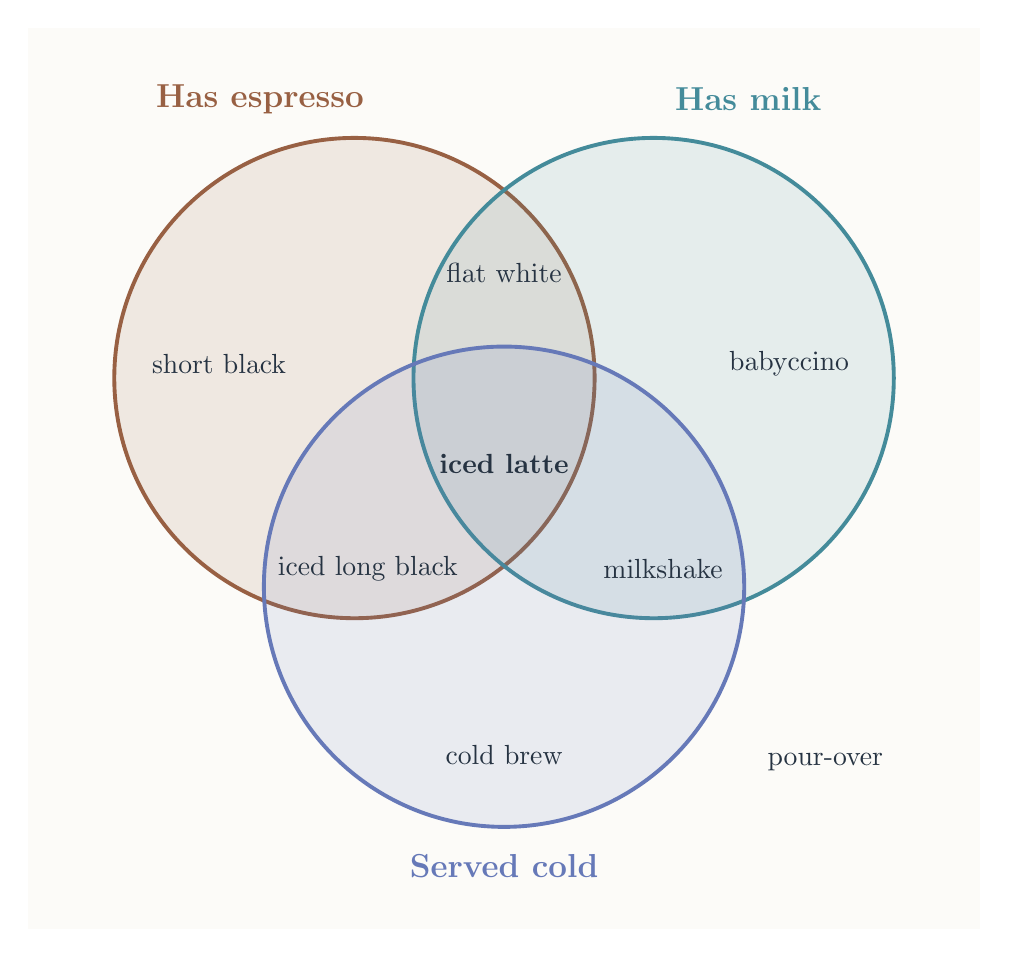
\begin{tikzpicture}[every node/.style={align=center}]
  \definecolor{ink}{HTML}{263342}
  \definecolor{espresso}{HTML}{986043}
  \definecolor{milk}{HTML}{448B9A}
  \definecolor{cold}{HTML}{6679B8}
  \definecolor{paper}{HTML}{FCFBF8}
  \fill[paper] (-6.05,-5.8) rectangle (6.05,5.65);
  % The three properties, with deliberately light washes so every intersection stays clear.
  \filldraw[fill=espresso,fill opacity=.12,draw=espresso,line width=1.4pt] (-1.9,1.2) circle (3.05);
  \filldraw[fill=milk,fill opacity=.12,draw=milk,line width=1.4pt] (1.9,1.2) circle (3.05);
  \filldraw[fill=cold,fill opacity=.12,draw=cold,line width=1.4pt] (0,-1.45) circle (3.05);
  % Labels are outside the circles to leave the small intersections uncluttered.
  \node[font=\bfseries\large,text=espresso] at (-3.1,4.74) {Has espresso};
  \node[font=\bfseries\large,text=milk] at (3.1,4.74) {Has milk};
  \node[font=\bfseries\large,text=cold] at (0,-5.00) {Served cold};
  % Espresso alone / milk alone / cold alone.
  \node[text=ink,font=\normalsize] at (-3.62,1.38) {short black};
  \node[text=ink,font=\normalsize] at (3.62,1.38) {babyccino};
  \node[text=ink,font=\normalsize] at (0,-3.58) {cold brew};
  % Pairwise intersections.
  \node[text=ink,font=\normalsize] at (0,2.54) {flat white};
  \node[text=ink,font=\normalsize] at (-1.73,-1.22) {iced long black};
  \node[text=ink,font=\normalsize] at (2.02,-1.22) {milkshake};
  % All three, and none of the above.
  \node[text=ink,font=\bfseries\normalsize] at (0,.11) {iced latte};
  \node[text=ink,font=\normalsize] at (4.08,-3.68) {pour-over};
\end{tikzpicture}
\end{document}
